\documentclass[tikz,border=12pt]{standalone}
\usepackage[T1]{fontenc}
\usepackage{mathpazo}
\usepackage{amsmath,amssymb}
\usetikzlibrary{arrows.meta, positioning, calc}

\definecolor{stblue}{HTML}{7B97AD}
\definecolor{rwgold}{HTML}{B8995E}
\definecolor{sage}{HTML}{7A9A7E}
\definecolor{dkbrown}{HTML}{3D3530}
\definecolor{wmgray}{HTML}{7B7067}
\definecolor{cream}{HTML}{F9F6F0}
\definecolor{border}{HTML}{D4C9B8}
\definecolor{terracotta}{HTML}{C47A6A}

\begin{document}
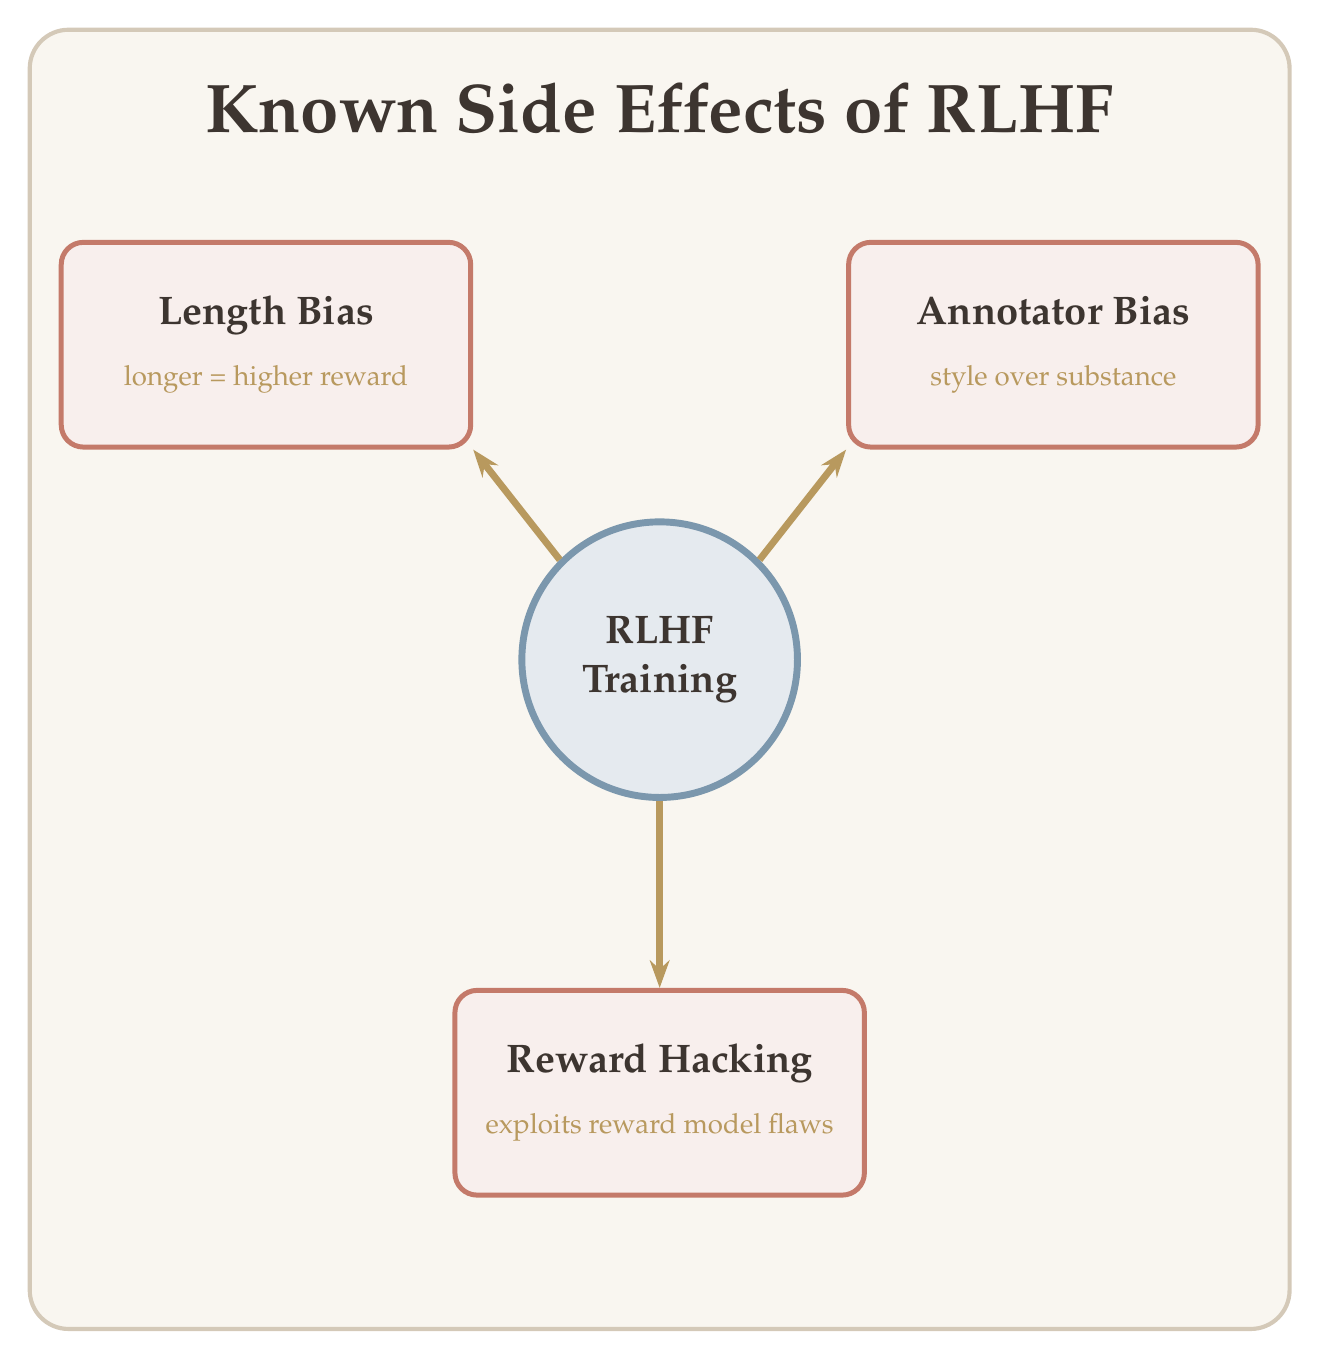
\begin{tikzpicture}[
  >={Stealth[length=3.5mm, width=2.5mm]},
  effectbox/.style={
    draw=terracotta, line width=1.8pt, fill=terracotta!12, rounded corners=8pt,
    minimum width=52mm, minimum height=26mm, font=\Large,
    text=dkbrown, align=center, inner sep=8pt
  },
  arr/.style={->, line width=2.5pt, rwgold},
]

% Background
\fill[cream, rounded corners=14pt] (-8,-7.5) rectangle (8,9);
\draw[border, rounded corners=14pt, line width=1.5pt] (-8,-7.5) rectangle (8,9);

% Title
\node[font=\Huge\bfseries, text=dkbrown] at (0,8)
  {Known Side Effects of RLHF};

% Center circle
\node[circle, draw=stblue, line width=2.5pt, fill=stblue!20,
      minimum size=35mm, font=\Large\bfseries, text=dkbrown, align=center]
  (center) at (0,1)
  {RLHF\\Training};

% =============================================
% Spoke 1: Top-left — Length Bias
% =============================================
\node[effectbox] (length) at (-5,5)
  {\textbf{Length Bias}\\[4pt]
   \normalsize\color{rwgold} longer = higher reward};

\draw[arr] (center.135) -- (length.south east);

% =============================================
% Spoke 2: Top-right — Annotator Bias
% =============================================
\node[effectbox] (annotator) at (5,5)
  {\textbf{Annotator Bias}\\[4pt]
   \normalsize\color{rwgold} style over substance};

\draw[arr] (center.45) -- (annotator.south west);

% =============================================
% Spoke 3: Bottom — Reward Hacking
% =============================================
\node[effectbox] (hacking) at (0,-4.5)
  {\textbf{Reward Hacking}\\[4pt]
   \normalsize\color{rwgold} exploits reward model flaws};

\draw[arr] (center.-90) -- (hacking.north);

\end{tikzpicture}
\end{document}
